\section{Results}

In this section, I report all the findings from the experiments, following the order of the research questions. Wherever possible, the original figures and tables are used to provide a clear overview.

\subsection{RQ1: Can a combined guardrail mechanism (RAG and moderator) ensure 100\% correctness in LLM responses to medical prompts?}

First of all, none of the tested guardrail methods managed to reach perfect (100\%) correctness. Table~\ref{tab:confusionmatrix} gives a breakdown of the confusion matrix for each model, as compared to the gold standard from manual review. For the combined approach, this means that out of 200 queries, 104 were correctly classified as true positives, while 36 correct answers were missed (false negatives).

\begin{table}[ht]
\centering
\caption{Confusion matrix per method. TP = True Positives, FN = False Negatives, TN = True Negatives, FP = False Positives.}
\label{tab:confusionmatrix}
\begin{tabular}{lcccc}
\toprule
Method & TP & FN & TN & FP \\
\midrule
RAG        & 109 & 31 & 28 & 31 \\
Moderator  & 133 & 7  & 9  & 50 \\
Combined   & 104 & 36 & 31 & 28 \\
\bottomrule
\end{tabular}
\end{table}

The bar chart in Figure~\ref{fig:prediction_performance_bar} shows at a glance how each method performed in terms of true/false positives and negatives.

\begin{figure}[ht]
  \centering
  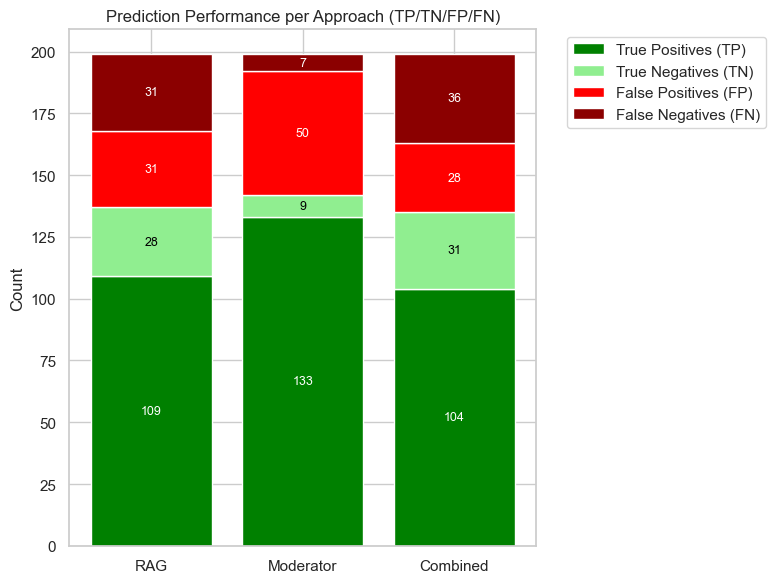
\includegraphics[width=0.95\linewidth]{figures/prediction_performance_per_approach.png}
  \caption{Prediction Performance per Approach, showing true positives, true negatives, false positives, and false negatives for RAG, Moderator, and Combined.}
  \label{fig:prediction_performance_bar}
\end{figure}

\subsection{RQ2: How was correctness operationalized for medication-related queries?}

To determine correctness, each model's answer was compared with the expert review. An answer counted as "correct" only if the medication, dosage, and indication matched what the expert considered appropriate for the specific patient. These criteria were used throughout for all performance calculations.

\subsection{RQ3: What are the strengths and limitations of each method in ensuring factual correctness?}

The key performance metrics are shown in Table~\ref{tab:metrics} and, for visual reference, in Figure~\ref{fig:model_performance_comparison_per_metric}. What stands out is that the Moderator approach reaches the highest recall (meaning it rarely misses a correct answer), while the Combined model has the highest precision (it makes the fewest false positive errors). RAG sits somewhere between the two.

\begin{table}[ht]
\centering
\caption{Performance metrics per method.}
\label{tab:metrics}
\begin{tabular}{lcccc}
\toprule
Method & Precision (\%) & Recall (\%) & F1-score (\%) & Accuracy (\%) \\
\midrule
RAG        & 77.9 & 77.9 & 77.9 & 68.8 \\
Moderator  & 72.7 & 95.0 & 82.4 & 71.4 \\
Combined   & 78.8 & 74.3 & 76.5 & 67.8 \\
\bottomrule
\end{tabular}
\end{table}

\begin{figure}[ht]
  \centering
  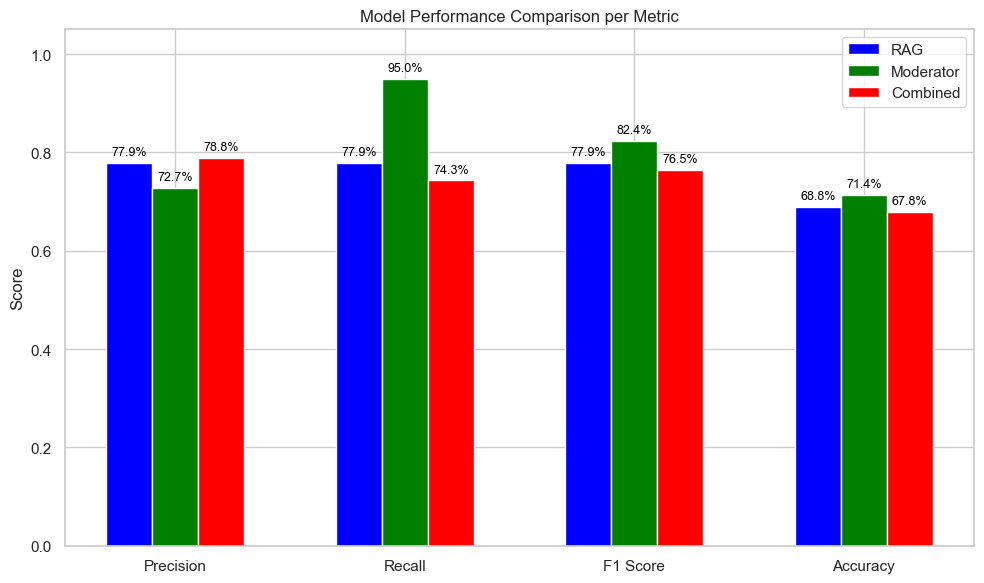
\includegraphics[width=0.95\linewidth]{figures/model_performance comparison_per_metric.png}
  \caption{Model Performance Comparison per Metric: precision, recall, F1 score, and accuracy for each model.}
  \label{fig:model_performance_comparison_per_metric}
\end{figure}

\subsection{Results on Individual Questions}

The detailed results per question are shown in Figure~\ref{fig:dna-results}. There were a few surprising cases: in 12 questions, both RAG and Moderator marked the answer as correct, but Combined did not. Conversely, there were 4 instances where RAG marked a response as incorrect, while Combined approved it. These are exceptions rather than the rule, but they show that the models do not always behave consistently.

\begin{figure}[ht]
    \centering
    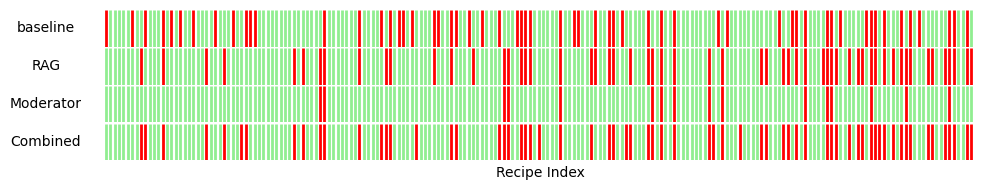
\includegraphics[width=1\linewidth]{figures/dna-results.png}
    \caption{Results on individual questions for each model, positive (green) and negative (red) answers.}
    \label{fig:dna-results}
\end{figure}

\subsection{Summary of Results}

In summary, while all three methods produced a substantial number of correct answers, none of them achieved perfect correctness. All main figures and tables are presented above, as required. Any further analysis or interpretation of these findings is left to the Discussion.